\documentclass[10pt,a4paper]{article}
\usepackage[T1]{fontenc}
\usepackage[utf8]{inputenc}
\usepackage{lmodern}
\usepackage{amsmath,amssymb,bm}
\usepackage[margin=17mm]{geometry}
\usepackage{graphicx,booktabs,tabularx,xcolor}
\usepackage{tikz}
\usetikzlibrary{arrows.meta,positioning,calc}
\usepackage{pdflscape}
\usepackage{fancyhdr}
\usepackage{hyperref}
\definecolor{navy}{HTML}{123047}
\definecolor{teal}{HTML}{087E8B}
\definecolor{light}{HTML}{EEF5F8}
\hypersetup{colorlinks=true,linkcolor=teal,urlcolor=teal}
\setlength{\parindent}{0pt}
\setlength{\parskip}{4pt}
\setlength{\headheight}{14pt}
\setlength{\abovedisplayskip}{5pt}
\setlength{\belowdisplayskip}{5pt}
\pagestyle{fancy}
\fancyhf{}
\fancyhead[L]{\small\textcolor{teal}{Research formulation: proposed method}}
\fancyfoot[L]{\scriptsize DHLCT-C2-60 / DIHOOL / Kinova Gen3 / CubeMars AK80}
\fancyfoot[R]{\thepage}
\renewcommand{\headrulewidth}{0.3pt}
\newcommand{\heading}[1]{\par\vspace{3pt}{\large\bfseries\color{teal}#1}\par}
\newcommand{\SE}{\mathrm{SE}}
\newcommand{\SO}{\mathrm{SO}}
\newcommand{\R}{\mathbb R}
\newcommand{\col}{\operatorname{col}}
\newcommand{\diag}{\operatorname{diag}}
\begin{document}
{\LARGE\bfseries\color{navy} ZMP-based stability of the mobile manipulator}\par
{\large Mechanical model and derivation of the stability measure}

\textbf{Aim.} Define a physically interpretable tipping-stability objective for coordinated base, lift, and arm motion. The formulation uses Newton--Euler dynamics and Lie-group kinematics; it does not assume a particular control algorithm.

\heading{1. System and mechanical inputs}
The configuration and generalized velocity are
\begin{align*}
q&=(G,s), &G&\in\SE(3), &s&=\col(h,\theta,\phi,\rho),\\
\nu&=\col(\xi_B,\dot s), &\xi_B&=\col(\omega_B,v_B), &\dot G&=G\widehat{\xi}_B.
\end{align*}
Here, $\col$ stacks its arguments into a column vector. $G$ is the chassis pose; $h$ is lift height; $\theta\in\R^7$ contains arm angles; $\phi\in\R^4$ contains driven wheel angles; and $\rho$ contains passive roller angles. Chassis angular and linear velocities, $\omega_B$ and $v_B$, are expressed in the chassis frame.

The coupled mechanical dynamics are
\begin{equation}
M(q)\dot\nu+c(q,\nu)+g_q(q)+d(q,\nu)
=B(q)u_{\mathrm{mech}}+J_c(q)^T\lambda_c.
\end{equation}
$M$ is generalized inertia, $c$ is the velocity-dependent inertial term, $g_q$ is gravity, $d$ is mechanical resistance, $B$ maps actuator effort, and $J_c$ is the contact Jacobian. The vector $\lambda_c$ contains ground-contact forces. The mechanical input is $u_{\mathrm{mech}}=\col(F_h,\tau_A,\tau_W)$: effective platform force, seven arm torques, and four wheel torques. Scissor-link motion is parameterized by $h$.

\heading{2. Whole-system Newton--Euler balance}
Total mass and centre of mass are
\begin{equation}
m=\sum_i m_i,\qquad p_C=\frac{1}{m}\sum_i m_i p_{C,i}.
\end{equation}
Angular momentum about the whole-system centre of mass is
\begin{equation}
H_C=\sum_i\left[R_iI_i\omega_i^B+
(p_{C,i}-p_C)\times m_i(\dot p_{C,i}-\dot p_C)\right].
\end{equation}
For component $i$, $m_i$ is mass, $p_{C,i}$ is its world centre of mass, $R_i$ is body-to-world rotation, $I_i$ is inertia about its centre of mass in its body frame, and $\omega_i^B$ is angular velocity in its own body frame. All terms in $H_C$ are expressed in the world frame.

Assuming gravity and ground contact are the only external loads,
\begin{equation}
F=m(\ddot p_C+g e_3),\qquad M_O=\dot H_C+p_C\times F.
\end{equation}
$F$ is total ground force, $M_O$ its moment about a fixed floor origin, $g$ gravitational acceleration, and $e_3=[0,0,1]^T$. An external tool wrench must be added when the arm interacts with the environment.

\heading{3. Zero-moment point on the floor}
For a horizontal floor at $z=0$, with $F_z>0$,
\begin{equation}
x_Z=-\frac{M_{O,y}}{F_z},\qquad y_Z=\frac{M_{O,x}}{F_z}.
\end{equation}
Writing $p_C=[x_C,y_C,z_C]^T$ gives
\begin{align}
x_Z&=x_C-\frac{z_Cm\ddot x_C+\dot H_{C,y}}{m(g+\ddot z_C)},\\
y_Z&=y_C-\frac{z_Cm\ddot y_C-\dot H_{C,x}}{m(g+\ddot z_C)}.
\end{align}
The ZMP is the floor point where the horizontal ground-wrench moment vanishes. It coincides with the centre of pressure for a valid planar contact solution. Lift height and arm motion enter through centre-of-mass acceleration and angular-momentum rate.

\newpage
{\LARGE\bfseries\color{navy} Stability objective and constraints}\par
{\large A compact formulation for an initial research proposal}

\heading{4. Express ZMP in the support frame}
Use a horizontal support frame $S$ centred on the wheel footprint, with axes aligned with chassis heading. Transform the world ZMP into that frame:
\begin{equation}
p_Z^S=R_2(\psi)^T(p_Z^W-o_S^W),\qquad
e_Z=p_Z^S-p_{Z,\mathrm{ref}}^S.
\end{equation}
$p_Z^W=[x_Z,y_Z]^T$, $R_2(\psi)$ is the planar rotation from $S$ to the world frame, $\psi$ is chassis heading, and $o_S^W$ is the footprint-centre position. The four-wheel support region is approximated by $[-a,a]\times[-b,b]$. The quantities $a,b$ are half the front--rear and left--right contact spacing, respectively; they are not the chassis dimensions.

\heading{5. Proposed stability cost}
Define the instantaneous cost
\begin{equation}
\ell_{\mathrm{stab}}=e_Z^TQ_Ze_Z,\qquad Q_Z=\diag(a^{-2},b^{-2}).
\end{equation}
Choosing the support centre as the reference, $p_{Z,\mathrm{ref}}^S=[0,0]^T$,
\begin{equation}
\boxed{\ell_{\mathrm{stab}}=
\left(\frac{x_Z^S}{a}\right)^2+
\left(\frac{y_Z^S}{b}\right)^2.}
\end{equation}
For a motion of duration $T$, use the average cost
\begin{equation}
\boxed{J_{\mathrm{stab}}=\frac{1}{T}\int_0^T\ell_{\mathrm{stab}}(t)\,dt
\simeq\frac{1}{N}\sum_{k=0}^{N-1}\ell_{\mathrm{stab},k}.}
\end{equation}
The discrete expression assumes $N$ equally spaced samples. Both costs are dimensionless. The cost is zero at the support centre and increases as the ZMP moves away. Footprint dimensions normalize both directions, so no independent tuning weights are needed in this initial formulation.

\heading{6. Feasibility and task requirements}
Keep a reserved distance $\delta$ from the support edges:
\begin{equation}
|x_Z^S|\le a-\delta,\qquad |y_Z^S|\le b-\delta,
\qquad 0<\delta<\min(a,b).
\end{equation}
The proposed command-selection problem is
\begin{equation}
\begin{aligned}
\min_{u_{\mathrm{cmd}}(\cdot)}\quad &J_{\mathrm{stab}}\\
\text{subject to}\quad &\text{system and inner-control dynamics},\\
&\text{required task motion and completion},\\
&\text{support, contact, collision, and actuator constraints}.
\end{aligned}
\end{equation}
The reserve $\delta$ accommodates estimation and model error. The cost encourages central support; the constraints preserve the reserve. Without task requirements, remaining stationary can minimize the stability cost.

If a wheel loses contact, replace the rectangle with the active contact polygon. ZMP containment alone does not prove recovery from arbitrary tilt or guarantee absence of slip. The controller method remains open.

\heading{Notation for the cost}
\renewcommand{\arraystretch}{1.2}
\begin{tabularx}{\linewidth}{@{}lXl@{}}
\toprule
Symbol & Definition & Units\\\midrule
$x_Z^S,y_Z^S$ & ZMP coordinates in the support frame & m\\
$a,b$ & Support half-length and half-width & m\\
$e_Z$ & ZMP error relative to the reference & m\\
$Q_Z$ & $\diag(1/a^2,1/b^2)$ & m$^{-2}$\\
$\delta$ & Reserved distance from each support edge & m\\
$T$ & Motion duration & s\\
$N,k$ & Sample count and sample index & --\\
\bottomrule
\end{tabularx}

\clearpage
\begin{landscape}
{\LARGE\bfseries\color{navy} Proposed hardware and feedback architecture}\par
{\large The robot image is the plant; controller choice remains open}

\begin{center}
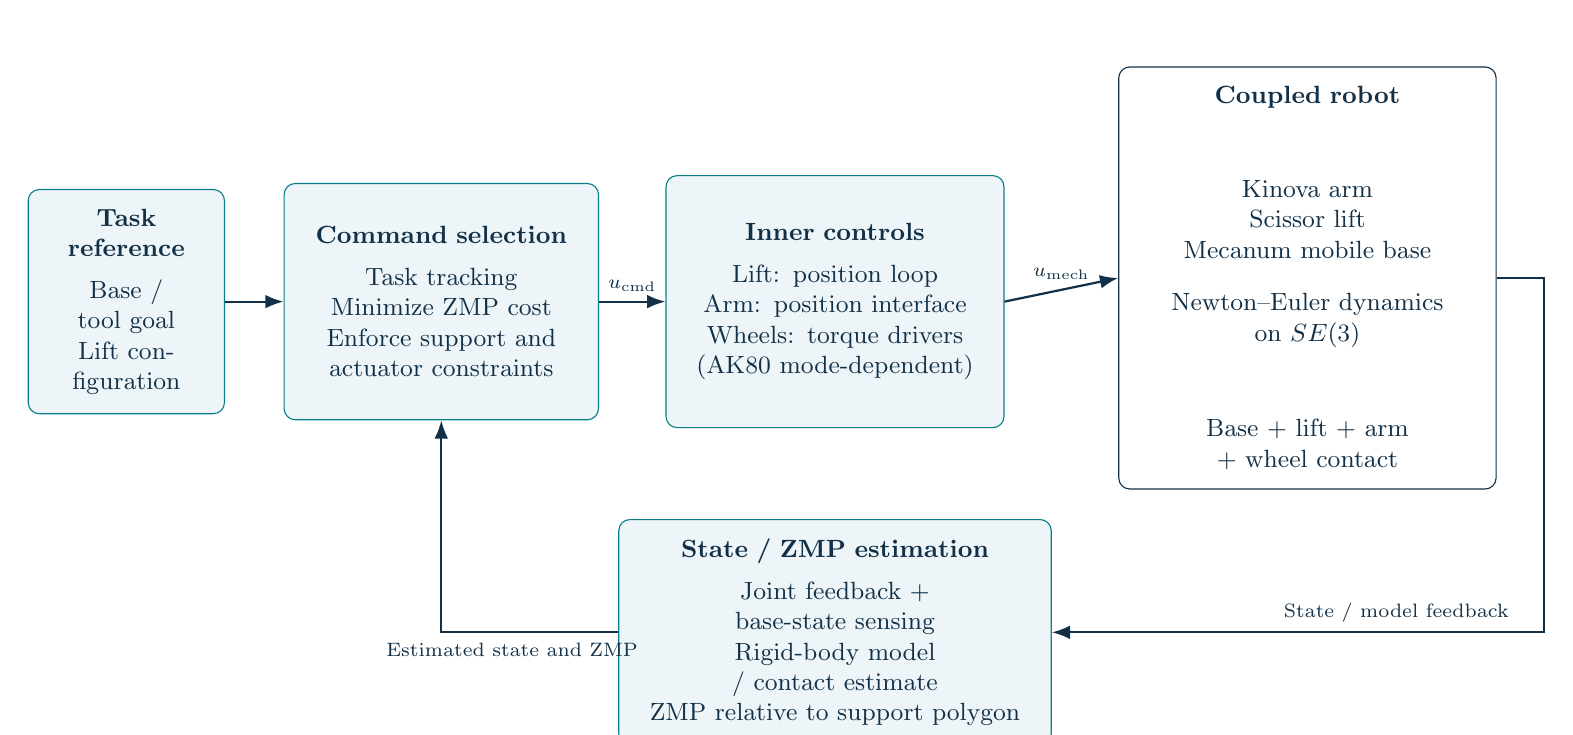
\begin{tikzpicture}[
 x=1cm,y=1cm,>=Latex,
 block/.style={draw=teal,rounded corners,fill=light,align=center,
   inner sep=7pt,font=\small,text=navy},
 signal/.style={->,thick,draw=navy},
 label/.style={font=\scriptsize,align=center,text=navy}]
\node[block,text width=2.0cm,minimum height=2cm] (task) at (0,0)
 {\textbf{Task reference}\\[4pt]Base / tool goal\\Lift configuration};
\node[block,text width=3.5cm,minimum height=3cm] (ctrl) at (4,0)
 {\textbf{Command selection}\\[4pt]Task tracking\\Minimize ZMP cost\\Enforce support and actuator constraints};
\node[block,text width=3.8cm,minimum height=3.2cm] (inner) at (9,0)
 {\textbf{Inner controls}\\[4pt]Lift: position loop\\Arm: position interface\\Wheels: torque drivers\\(AK80 mode-dependent)};
\node[block,draw=navy,fill=white,text width=4.3cm,minimum height=5.1cm] (robot) at (15,0.3)
 {\textbf{Coupled robot}\\[4pt]
 % With the companion PNG beside this file, the original robot appears here.
 % The fallback keeps this source compilable in single-file LaTeX editors.
 \IfFileExists{robot_reference.png}{\includegraphics[height=3.6cm]{robot_reference.png}}{
 \parbox[c][3.6cm][c]{4cm}{\centering Kinova arm\\Scissor lift\\Mecanum mobile base\\[8pt]Newton--Euler dynamics\\on $SE(3)$}}
 \\[4pt]Base + lift + arm + wheel contact};
\node[block,text width=5cm,minimum height=2cm] (estimate) at (9,-4.2)
 {\textbf{State / ZMP estimation}\\[4pt]Joint feedback + base-state sensing\\Rigid-body model / contact estimate\\ZMP relative to support polygon};
\draw[signal] (task.east)--(ctrl.west);
\draw[signal] (ctrl.east)--node[label,above] {$u_{\mathrm{cmd}}$}(inner.west);
\draw[signal] (inner.east)--node[label,above] {$u_{\mathrm{mech}}$}(robot.west);
\draw[signal] (robot.east)--++(0.6,0)|-node[label,pos=.65,above]{State / model feedback}(estimate.east);
\draw[signal] (estimate.west)-|node[label,pos=.3,below]{Estimated state and ZMP}(ctrl.south);
\end{tikzpicture}
\end{center}

\textbf{Hardware command:}
$u_{\mathrm{cmd}}=\col(a_{\mathrm{ref}},\theta_{\mathrm{ref}},\tau_{W,\mathrm{ref}})$ contains the actuator-extension target, arm-position targets, and wheel-torque targets. The lift potentiometer closes its position loop; it does not measure force. Torque-controlled wheels assume a compatible AK80 driver mode. Inner controls produce the mechanical force/torque inputs used in the dynamics.

\textbf{Implementation status:} this diagram defines a proposed architecture, not a claim that the stability controller or contact-force estimator has already been implemented or validated.
\end{landscape}
\end{document}
